%package list
\documentclass{article}
\usepackage[top=3cm, bottom=3cm, outer=3cm, inner=3cm]{geometry}
\usepackage{graphicx}
\usepackage{url}
%\usepackage{cite}
\usepackage{hyperref}
\usepackage{array}
\usepackage{multicol}
\newcolumntype{x}[1]{>{\centering\arraybackslash\hspace{0pt}}p{#1}}
\usepackage{natbib}
\usepackage{pdfpages}
\usepackage{multirow}
\usepackage{float}
\usepackage[normalem]{ulem}
\useunder{\uline}{\ul}{}
\usepackage{svg}
\usepackage{amsmath}
\usepackage{hyperref}

%%%%%%%%%%%%%%%%%%%%%%%%%%%%%%%%%%%%%%%%%%%%%%%%%%%%%%%%%%%%%%%%%%%%%%%%%%%%
%%%%%%%%%%%%%%%%%%%%%%%%%%%%%%%%%%%%%%%%%%%%%%%%%%%%%%%%%%%%%%%%%%%%%%%%%%%%
\newcommand{\csemail}{vmachacaa@unsa.edu.pe}
\newcommand{\csdocente}{Vicente Machaca Arceda}
\newcommand{\cscurso}{Algoritmos y Estructura de Datos}
\newcommand{\csuniversidad}{Universidad Nacional de San Agustín}
\newcommand{\csescuela}{Maestría en Ciencias de la Computación}
\newcommand{\cspracnr}{04}
\newcommand{\cstema}{Kd-tree}
%%%%%%%%%%%%%%%%%%%%%%%%%%%%%%%%%%%%%%%%%%%%%%%%%%%%%%%%%%%%%%%%%%%%%%%%%%%%
%%%%%%%%%%%%%%%%%%%%%%%%%%%%%%%%%%%%%%%%%%%%%%%%%%%%%%%%%%%%%%%%%%%%%%%%%%%%


\usepackage[english,spanish]{babel}
\usepackage[utf8]{inputenc}
\AtBeginDocument{\selectlanguage{spanish}}
\renewcommand{\figurename}{Figura}
\renewcommand{\refname}{Referencias}
\renewcommand{\tablename}{Tabla} %esto no funciona cuando se usa babel
\AtBeginDocument{%
	\renewcommand\tablename{Tabla}
}

\usepackage{fancyhdr}
\pagestyle{fancy}
\fancyhf{}
\setlength{\headheight}{30pt}
\renewcommand{\headrulewidth}{1pt}
\renewcommand{\footrulewidth}{1pt}
\fancyhead[L]{\raisebox{-0.2\height}{
\includegraphics[width=3cm]{img/logo_unsa}}}
\fancyhead[C]{}
\fancyhead[R]{\fontsize{7}{7}\selectfont	\csuniversidad \\ \csescuela \\ \textbf{\cscurso} }
\fancyfoot[L]{Grupo N◦ 02}
\fancyfoot[C]{\cscurso}
\fancyfoot[R]{Página \thepage}

\begin{document}

\vspace*{10px}

\begin{center}
	\fontsize{17}{17} \textbf{ Práctica \cspracnr}
\end{center}

%\centerline{\textbf{\underline{\Large Título: Informe de revisión del estado del arte}}}
%\vspace*{0.5cm}

\begin{table}[h]
	\begin{tabular}{|x{4.7cm}|x{4.8cm}|x{4.8cm}|}
		\hline
		\textbf{DOCENTE} & \textbf{CARRERA} & \textbf{CURSO} \\
		\hline
		\csdocente       & \csescuela       & \cscurso       \\
		\hline
	\end{tabular}
\end{table}

\begin{table}[h]
	\begin{tabular}{|x{4.7cm}|x{4.8cm}|x{4.8cm}|}
		\hline
		\textbf{PRÁCTICA} & \textbf{TEMA} & \textbf{DURACIÓN} \\
		\hline
		\cspracnr         & \cstema       & --                \\
		\hline
	\end{tabular}
\end{table}

\section{Integrantes}
\begin{itemize}
	\item Grupo N° 2
	\item Integrantes:
	      \begin{itemize}
		      \item EDER ALONSO AMPUERO ATAMARI
		      \item HOWARD FERNANDO ARANZAMENDI MORALES
		      \item JOSE EDISON PEREZ MAMANI
		      \item HENRRY IVAN ARIAS MAMANI
	      \end{itemize}
\end{itemize}

\section{Repositorio GitHub}
URL Github: \href{https://github.com/hAriasm/Practica4_ayed}{Repositorio Práctica 4 AyED}

\section{Marco Teórico}
\subsection{Kd-Tree}

\subsubsection{Definición}
\paragraph{}
Un KD-Tree (también llamado árbol K-dimensional) es un árbol de búsqueda binaria donde los datos en cada nodo son un punto K-dimensional en el espacio. En resumen, es una estructura de datos de partición de espacio (detalles a continuación) para organizar puntos en un espacio K-Dimensional.

Un nodo que no es una hoja en el árbol K-D divide el espacio en dos partes, llamadas medios espacios.

Los puntos a la izquierda de este espacio están representados por el subárbol izquierdo de ese nodo y los puntos a la derecha del espacio están representados por el subárbol derecho. Pronto estaremos explicando el concepto de cómo se divide el espacio y se forma el árbol.

En aras de la simplicidad, entendamos un árbol 2-D con un ejemplo.

La raíz tendría un plano alineado con el eje x, los hijos de la raíz tendrían ambos planos alineados con el eje y, los nietos de la raíz tendrían todos planos alineados con el eje x, y los bisnietos de la raíz tendrían todos planos alineados con el eje y, y así sucesivamente.

\subsubsection{Generalización}
\paragraph{}
Numeremos los planos como 0, 1, 2, …(K – 1). Del ejemplo anterior, es bastante claro que un punto (nodo) en la profundidad D tendrá un plano alineado donde A se calcula como:

A = D mod K

\subsubsection{¿Cómo determinar si un punto estará en el subárbol izquierdo o en el subárbol derecho?}
\paragraph{}
Si el nodo raíz esta alineado en el plano A, el subárbol izquierdo contendrá todos los puntos cuyas coordenadas en ese plano sean más pequeñas que las del nodo ráiz. De manera similar, el subárbol derecho contendrá todos los puntos cuyas coordenadas en ese plano sean mayores-iguales que las del nodo raíz.

\subsubsection{Creación de un árbol 2-D}
\paragraph{}
Considere los siguientes puntos en un plano 2-D:
(3, 6), (17, 15), (13, 15), (6, 12), (9, 1), (2, 7), (10, 19)

\begin{enumerate}
	\item Insertar (3, 6): dado que el árbol está vacío, conviértalo en el nodo raíz.
	\item Insertar (17, 15): compararlo con el punto del nodo raíz. Dado que el nodo raíz está alineado con X, el valor de la coordenada X se comparará para determinar si se encuentra en el subárbol derecho o en el subárbol izquierdo. Este punto estará alineado con Y.
	\item Insertar (13, 15): el valor X de este punto es mayor que el valor X del punto en el nodo raíz. Entonces, esto estará en el subárbol derecho de (3, 6). Nuevamente compare el valor Y de este punto con el valor Y del punto (17, 15) (¿Por qué?). Como son iguales, este punto estará en el subárbol derecho de (17, 15). Este punto estará alineado con X.
	\item Insertar (6, 12): el valor X de este punto es mayor que el valor X del punto en el nodo raíz. Entonces, esto estará en el subárbol derecho de (3, 6). Nuevamente compare el valor Y de este punto con el valor Y del punto (17, 15) (¿Por qué?). Como 12 < 15, este punto estará en el subárbol izquierdo de (17, 15). Este punto estará alineado con X.
	\item Insertar (9, 1): De manera similar, este punto estará a la derecha de (6, 12).
	\item Insertar (2, 7): De manera similar, este punto estará a la izquierda de (3, 6).
	\item Inserta (10, 19): De manera similar, este punto estará a la izquierda de (13, 15).
\end{enumerate}

\begin{figure}[h!]
	\centering
	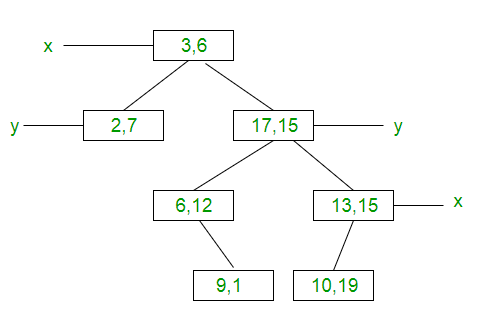
\includegraphics[width=0.8\textwidth]{img/kdtree_1.png}
	\caption{Nodos en KDTREE}
	\label{fig:kdtree_01}
\end{figure}

\subsubsection{¿Cómo se divide el espacio?}
\paragraph{}
Los 7 puntos se trazarán en el plano X-Y de la siguiente manera:

\begin{enumerate}
	\item El punto (3, 6) dividirá el espacio en dos partes: Dibujar la línea X = 3.
	\item El punto (2, 7) dividirá el espacio a la izquierda de la línea X = 3 en dos partes horizontalmente. Dibuja la línea Y = 7 a la izquierda de la línea X = 3.
	\item El punto (17, 15) dividirá el espacio a la derecha de la línea X = 3 en dos partes horizontalmente. Dibuja la línea Y = 15 a la derecha de la línea X = 3.
	\item El punto (6, 12) dividirá el espacio debajo de la línea Y = 15 ya la derecha de la línea X = 3 en dos partes. Dibuja la línea X = 6 a la derecha de la línea X = 3 y debajo de la línea Y = 15.
	\item El punto (13, 15) dividirá el espacio debajo de la línea Y = 15 ya la derecha de la línea X = 6 en dos partes. Dibuja la línea X = 13 a la derecha de la línea X = 6 y debajo de la línea Y = 15.
	\item El punto (9, 1) dividirá el espacio entre las líneas X = 3, X = 6 e Y = 15 en dos partes. Dibuja la línea Y = 1 entre las líneas X = 3 y X = 13.
	\item El punto (10, 19) dividirá el espacio a la derecha de la línea X = 3 y arriba de la línea Y = 15 en dos partes. Dibuja la línea Y = 19 a la derecha de la línea X = 3 y arriba de la línea Y = 15.
\end{enumerate}

\begin{figure}[h!]
	\centering
	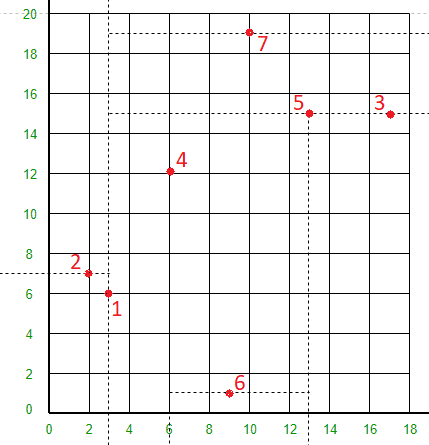
\includegraphics[width=0.8\textwidth]{img/kdtree_2.png}
	\caption{División del espacio en KD-TREE}
	\label{fig:kdtree_02}
\end{figure}

\subsection{KNN}
\subsubsection{Definición}
\paragraph{}
K-Nearest Neighbors es uno de los algoritmos de clasificación más básicos pero esenciales en Machine Learning. Pertenece al dominio de aprendizaje supervisado y encuentra una intensa aplicación en el reconocimiento de patrones, minería de datos y detección de intrusos.
Es ampliamente disponible en escenarios de la vida real ya que no es paramétrico, lo que significa que no hace suposiciones subyacentes sobre la distribución de datos (a diferencia de otros algoritmos como GMM, que asume una distribución gaussiana de los datos dados) .
Nos dan unos datos previos (también llamados datos de entrenamiento), que clasifican las coordenadas en grupos identificados por un atributo.
Como ejemplo, considere la siguiente tabla de puntos de datos que contienen dos características:

\begin{figure}[h!]
	\centering
	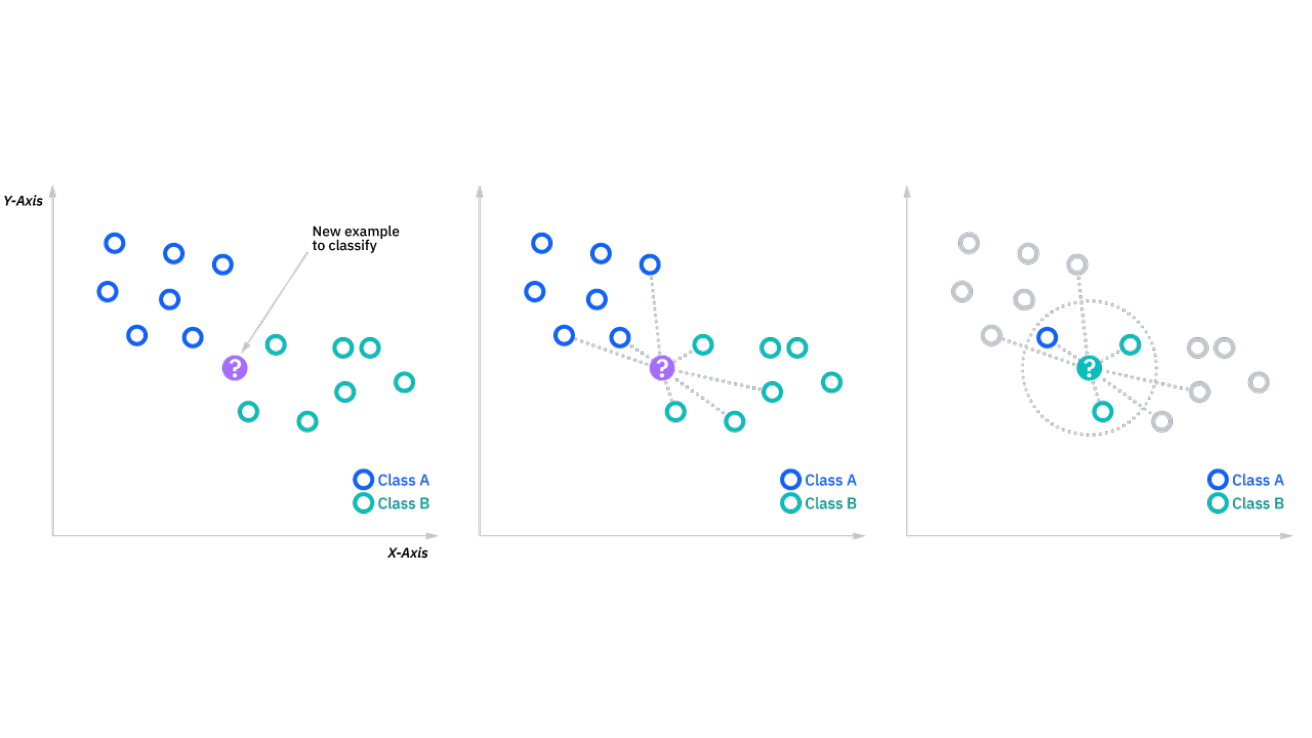
\includegraphics[width=0.8\textwidth]{img/knn_01.png}
	\caption{División del espacio en KD-TREE}
	\label{fig:knn_01}
\end{figure}

Ahora, dado otro conjunto de puntos de datos (también llamados datos de prueba), asigne estos puntos a un grupo analizando el conjunto de entrenamiento. Tenga en cuenta que los puntos no clasificados están marcados como 'Blanco'.

\begin{figure}[h!]
	\centering
	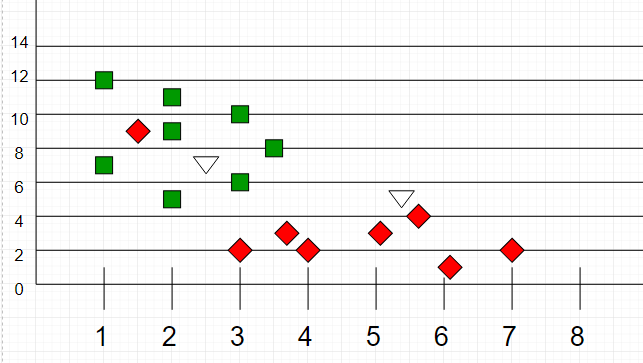
\includegraphics[width=0.8\textwidth]{img/knn_02.png}
	\caption{División del espacio en KD-TREE}
	\label{fig:knn_02}
\end{figure}

\subsubsection{Intuición}
Si trazamos estos puntos en un gráfico, podemos ubicar algunos grupos o grupos. Ahora, dado un punto sin clasificar, podemos asignarlo a un grupo observando a qué grupo pertenecen sus vecinos más cercanos. Esto significa que un punto cercano a un grupo de puntos clasificados como "Rojo" tiene una mayor probabilidad de ser clasificado como "Rojo".
Intuitivamente, podemos ver que el primer punto (2.5, 7) debe clasificarse como 'Verde' y el segundo punto (5.5, 4.5) debe clasificarse como 'Rojo'.

\subsubsection{Algoritmo}
Sea m el número de muestras de datos de entrenamiento. Sea p un punto desconocido.

\begin{enumerate}
	\item Almacene las muestras de entrenamiento en una matriz de puntos de datos arr[]. Esto significa que cada elemento de esta matriz representa una tupla (x, y).
	\item Haz el conjunto S de las K distancias más pequeñas obtenidas. Cada una de estas distancias corresponde a un punto de datos ya clasificado.
	\item Devuelve la etiqueta mayoritaria entre S.
\end{enumerate}

\paragraph{}
K se puede mantener como un número impar para que podamos calcular una clara mayoría en el caso de que solo sean posibles dos grupos (por ejemplo, rojo/azul). Con el aumento de K, obtenemos límites más suaves y definidos a través de diferentes clasificaciones. Además, la precisión del clasificador anterior aumenta a medida que aumentamos la cantidad de puntos de datos en el conjunto de entrenamiento.

\section{Ejercicios}

\subsection{Ejercicio N° 1}
El la imagen \ref{fig:ejercicio_01} se presenta la creación del archivo html.
\begin{figure}[h!]
	\centering
	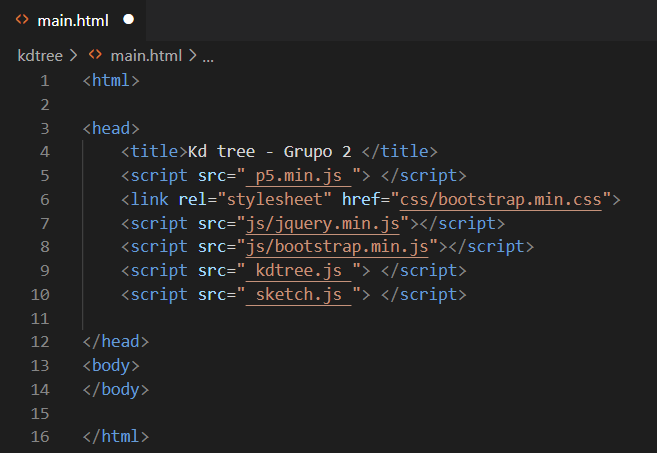
\includegraphics[width=0.8\textwidth]{img/ejercicio_01.png}
	\caption{Archivo html}
	\label{fig:ejercicio_01}
\end{figure}

\subsection{Ejercicio N° 2}
\subsection{Ejercicio N° 3}
\subsection{Ejercicio N° 4}
\subsection{Ejercicio N° 5}
\begin{figure}[h!]
El la imagen \ref{fig:ejercicio_05_1} se muestra el resultado de la implementación de la función closest_point_brute_force y en la imagen \ref{fig:ejercicio_05_2} se muestra el resultado de la implementacion de la función naive_closest_point.
	\centering
	\includegraphics[width=0.8\textwidth]{img/ejercicio_05_1.png}
	\caption{Función closest_point_brute_force}
	\label{fig:ejercicio_05_1}
\end{figure}

\begin{figure}[h!]
	\centering
	\includegraphics[width=0.8\textwidth]{img/ejercicio_05_2.png}
	\caption{Función naive_closest_point}
	\label{fig:ejercicio_05_2}
\end{figure}

\subsection{Ejercicio N° 6}
El la imagen \ref{fig:ejercicio_06_1} se muestra el resultado de la implementación de la función closest_point_brute_force y en la imagen \ref{fig:ejercicio_06_2} se muestra el resultado de la implementacion de la función naive_closest_point.
\begin{figure}[h!]
	\centering
	\includegraphics[width=0.8\textwidth]{img/ejercicio_06_1.png}
	\caption{Función closest_point_brute_force}
	\label{fig:ejercicio_06_1}
\end{figure}

\begin{figure}[h!]
	\centering
	\includegraphics[width=0.8\textwidth]{img/ejercicio_06_2.png}
	\caption{Función naive_closest_point}
	\label{fig:ejercicio_06_2}
\end{figure}

\subsection{Ejercicio N° 7}
El la imagen \ref{fig:ejercicio_07} se muestra el resultado de la implementación de la función closest_point.
\begin{figure}[h!]
	\centering
	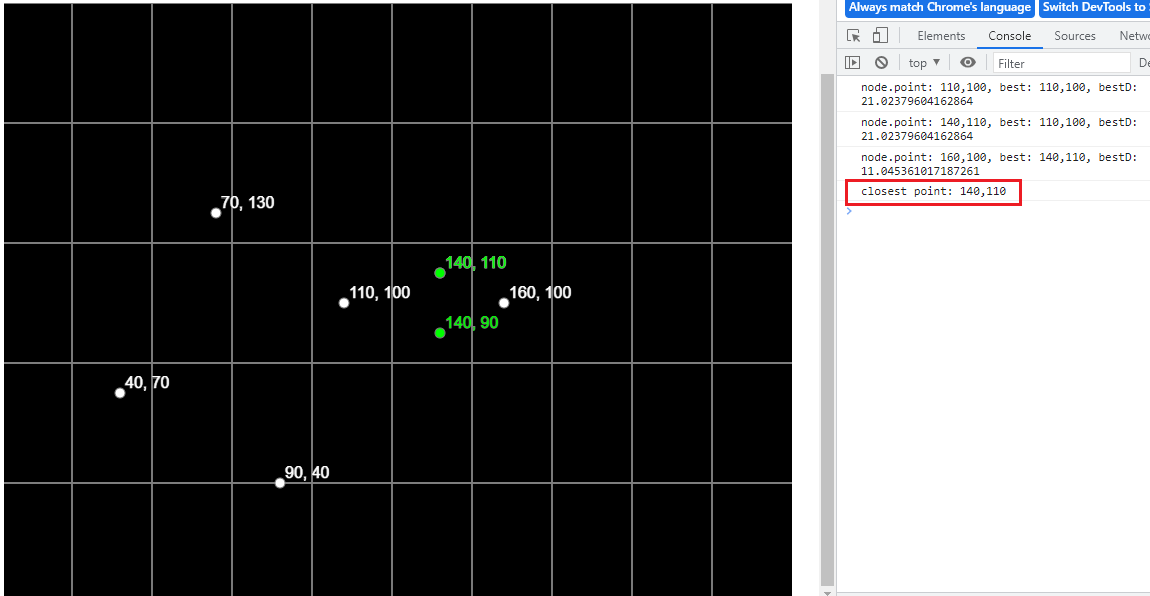
\includegraphics[width=0.8\textwidth]{img/ejercicio_07.png}
	\caption{Función closest_point}
	\label{fig:ejercicio_07}
\end{figure}


\subsection{Ejercicio N° 8}
El la imagen \ref{fig:ejercicio_08} se muestra el resultado de la implementación de la función KNN, que retorna los k puntos mas cercanos a un punto.
\begin{figure}[h!]
	\centering
	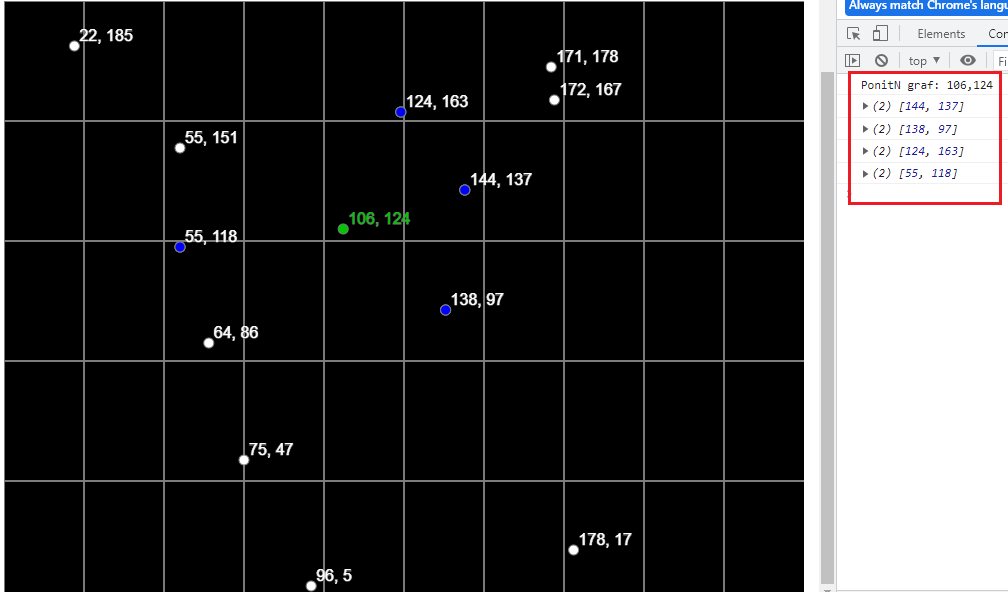
\includegraphics[width=0.8\textwidth]{img/ejercicio_08.png}
	\caption{Función KNN, que retorna k puntos mas cercanos}
	\label{fig:ejercicio_08}
\end{figure}

\subsection{Ejercicio N° 9}
El la imagen \ref{fig:ejercicio_09} se muestra el resultado de la implementación de la función range_query_circle de KD-Tree
\begin{figure}[h!]
	\centering
	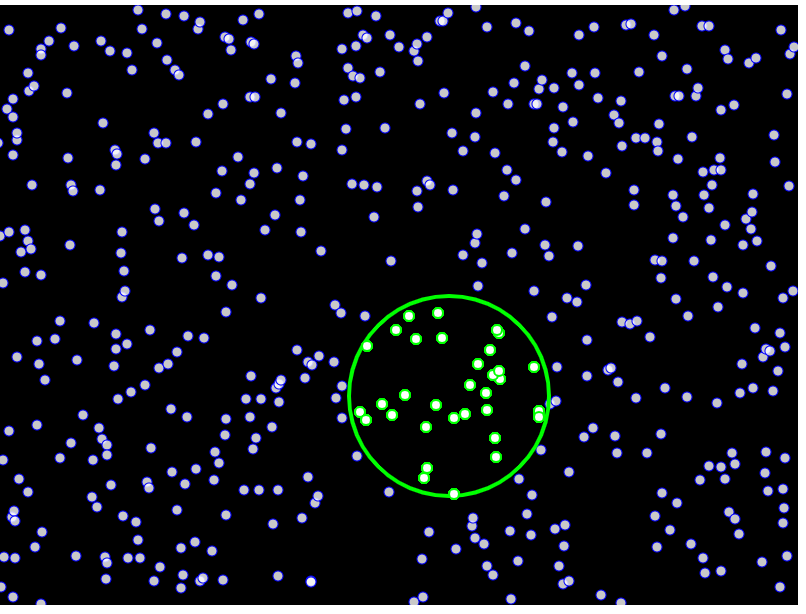
\includegraphics[width=0.8\textwidth]{img/ejercicio_09.png}
	\caption{Función range_query_circle de KD-Tree}
	\label{fig:ejercicio_09}
\end{figure}

\subsection{Ejercicio N° 10}
El la imagen \ref{fig:ejercicio_10} se muestra el resultado de la implementación de la función range_query_rec de KD-Tree
\begin{figure}[h!]
	\centering
	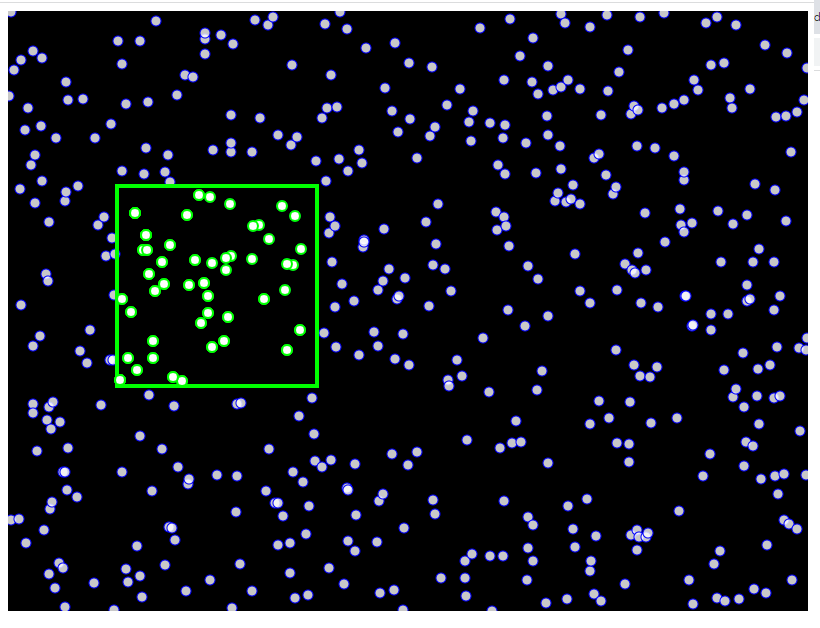
\includegraphics[width=0.8\textwidth]{img/ejercicio_10.png}
	\caption{Función range_query_rec de KD-Tree}
	\label{fig:ejercicio_10}
\end{figure}

\clearpage
\section{Conclusiones}
\begin{itemize}
	\item El quadtree se codifican en un árbol de cuatro hijos no balanceado, y el  octree se codifica en un árbol octal no balanceado.
	\item De la bibliografía revisada, se concluye que las aplicaciones más comunes para los QuadTree y OcTree son el Procesamiento de imágenes, generación de mallas e indexado espacial.
	\item Las estructuras octree son usadas mayormente para partir un espacio tridimensional, dividiéndolo recursivamente en ocho octantes, siendo análogas tridimensionales de los quadtree bidimensionales.
\end{itemize}

\section{Referencias}
\begin{enumerate}
	\item Amalia Duch, Vladimir Estivill-Castro, Conrado Martínez, “Randomized K-Dimensional Binary Seach Trees”, M-RR/LSI-98-48-R, Universitat Politècnica de Catalunya, Barcelona, 1998.
	\item C. Martínez y S. Roura, “Randomized binary search trees”, Journal of the ACM, Marzo 1998, Volumen 45, núm. 2, 288$–$323.
	\item W. Cunto, G. Lau, y Ph. Flajolet, “Analysis of kd-trees: kd-trees improved by local reorganizations”, In F. Dehne, J. R. Sack y N. Santoro editors, Work, Algorithms and Data Structures, 1989, Volumen 382, 24$–$38.
	\item Andrew W. Moore, “An Introductory tutorial on kd-trees”, Carnegie Mellon University, awm@cs.cmu.edu, 1992. http://www.autonlab.org.
	\item Luc Devroye, Nicholas Broutin, Ketan Dalal y Erin McLeish, “The kdtreap”, Personal Communication.
	\item \href{https://p5js.org/es/libraries/}{P5.js}
	\item \href{https://www.geeksforgeeks.org/}{Geeksforgeeks}
\end{enumerate}

\end{document}
